\documentclass[border=3pt]{standalone}
% Preâmbulo compartilhado pelos diagramas TikZ da aula 10 (Localização de Markov e Gaussiana)
\usepackage[T1]{fontenc}
\usepackage[utf8]{inputenc}
\usepackage{lmodern}
\usepackage{amsmath}
\usepackage{xcolor}
\usepackage{tikz}
\usetikzlibrary{arrows.meta,angles,quotes,decorations.pathmorphing,calc,
                positioning,shapes.geometric,shapes.misc,backgrounds,fit,
                math}

% Paleta (mesma dos SVGs originais)
\definecolor{dblue}{HTML}{2A5B8C}
\definecolor{dorange}{HTML}{B3541E}
\definecolor{dgreen}{HTML}{4A7C59}
\definecolor{dred}{HTML}{9C4B4B}
\definecolor{dcream}{HTML}{F4F1EA}
\definecolor{dshade}{HTML}{DDD7C9}

% Função gaussiana (não normalizada por padrão de escala visual)
\pgfmathdeclarefunction{gauss}{3}{%
  \pgfmathparse{1/(#3*sqrt(2*pi))*exp(-((#1-#2)^2)/(2*#3^2))}%
}

% Estilos comuns (prefixo d... para não colidir com chaves internas do pgf)
\tikzset{
  >={Stealth[length=2mm]},
  dguide/.style={gray!55, dashed, line width=0.4pt},
  daxis/.style={gray!60, line width=0.7pt, ->},
  dbody/.style={fill=black!3, draw=black!80, line width=1pt},
  dacc/.style={draw=dblue, line width=1pt},
  dlbl/.style={black!55, font=\small},
  dsub/.style={black!45, font=\footnotesize},
  dstate/.style={circle, draw=black!80, fill=dcream, line width=1pt,
                 minimum size=17mm, font=\large, inner sep=1pt},
  dobs/.style={circle, draw=black!80, fill=dshade, line width=1pt,
               minimum size=14mm, font=\large, inner sep=1pt},
  dbox/.style={rounded corners=2pt, draw=black!80, fill=dcream, line width=1pt,
               align=center, inner sep=6pt},
  dop/.style={circle, draw=black!80, fill=white, line width=1pt,
              minimum size=6mm, inner sep=0pt, font=\small},
  dtrans/.style={->, dblue, line width=1pt},
  dmeas/.style={->, dorange, line width=1pt},
  dcurve/.style={line width=1pt, dblue},
  dcurveb/.style={line width=1.4pt, dorange},
}

\usetikzlibrary{shapes.callouts}
\begin{document}
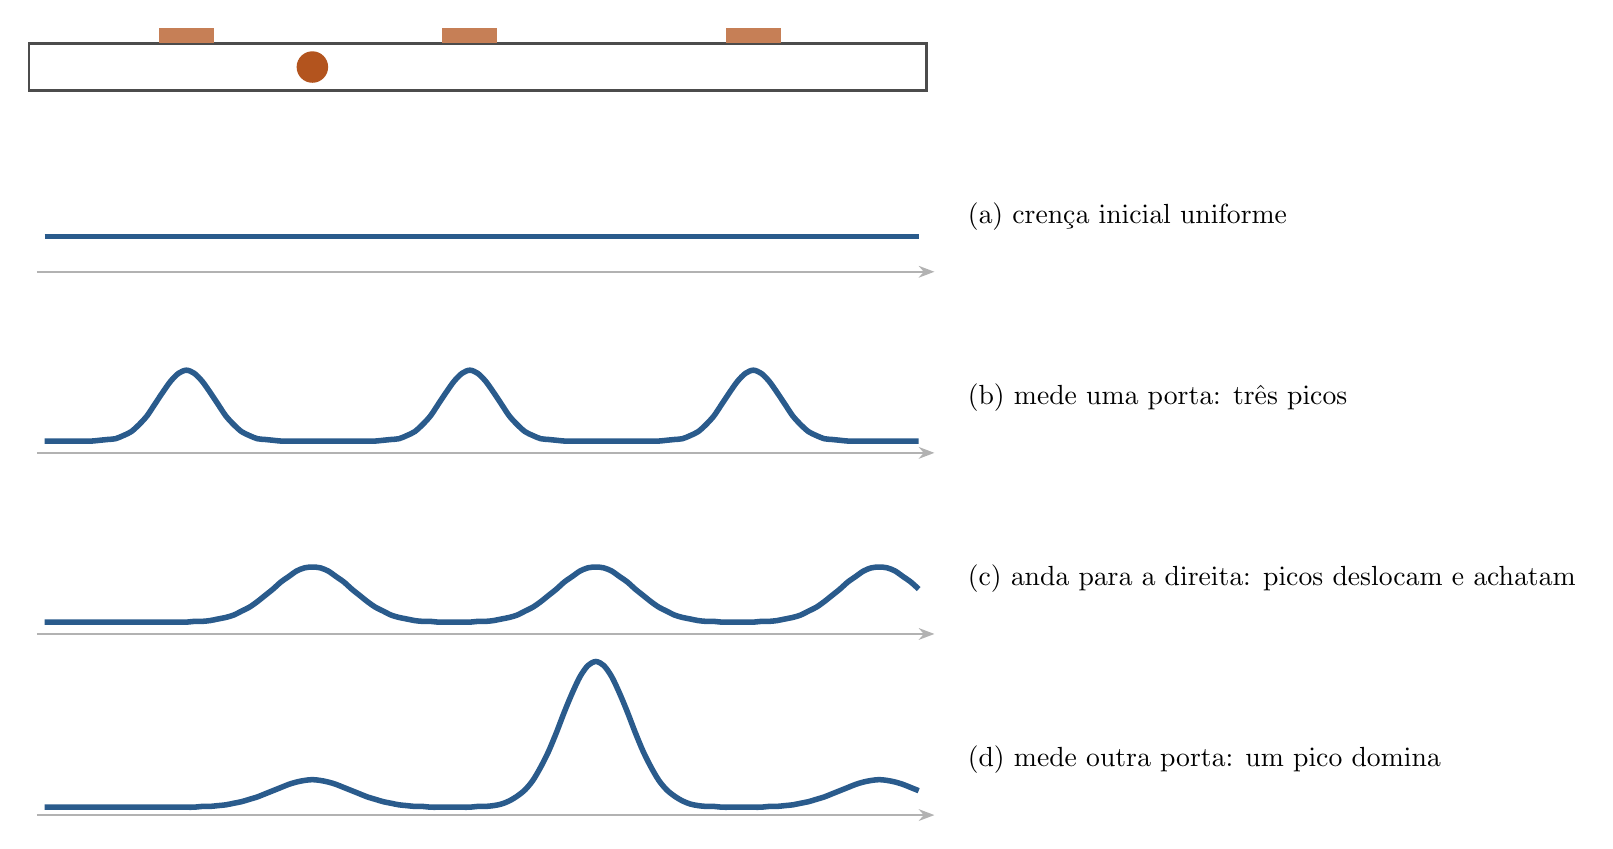
\begin{tikzpicture}[x=1cm,y=1cm,bal/.style={rectangle callout, rounded corners=7pt, draw=black!75, fill=white, line width=1pt, align=center, font=\normalsize, inner sep=5pt}]
\draw[black!70, fill=white, line width=0.9pt] (0,9.70) rectangle (11.4,10.30);
\fill[dorange!75] (1.65,10.30) rectangle (2.35,10.50);
\fill[dorange!75] (5.25,10.30) rectangle (5.95,10.50);
\fill[dorange!75] (8.85,10.30) rectangle (9.55,10.50);
\fill[dorange] (3.60,10.00) circle (0.2);
\draw[daxis] (0.1,7.40) -- (11.5,7.40);
\draw[dblue, line width=2pt] plot[smooth] coordinates {(0.20,7.85) (0.30,7.85) (0.40,7.85) (0.50,7.85) (0.60,7.85) (0.70,7.85) (0.80,7.85) (0.90,7.85) (1.00,7.85) (1.10,7.85) (1.20,7.85) (1.30,7.85) (1.40,7.85) (1.50,7.85) (1.60,7.85) (1.70,7.85) (1.80,7.85) (1.90,7.85) (2.00,7.85) (2.10,7.85) (2.20,7.85) (2.30,7.85) (2.40,7.85) (2.50,7.85) (2.60,7.85) (2.70,7.85) (2.80,7.85) (2.90,7.85) (3.00,7.85) (3.10,7.85) (3.20,7.85) (3.30,7.85) (3.40,7.85) (3.50,7.85) (3.60,7.85) (3.70,7.85) (3.80,7.85) (3.90,7.85) (4.00,7.85) (4.10,7.85) (4.20,7.85) (4.30,7.85) (4.40,7.85) (4.50,7.85) (4.60,7.85) (4.70,7.85) (4.80,7.85) (4.90,7.85) (5.00,7.85) (5.10,7.85) (5.20,7.85) (5.30,7.85) (5.40,7.85) (5.50,7.85) (5.60,7.85) (5.70,7.85) (5.80,7.85) (5.90,7.85) (6.00,7.85) (6.10,7.85) (6.20,7.85) (6.30,7.85) (6.40,7.85) (6.50,7.85) (6.60,7.85) (6.70,7.85) (6.80,7.85) (6.90,7.85) (7.00,7.85) (7.10,7.85) (7.20,7.85) (7.30,7.85) (7.40,7.85) (7.50,7.85) (7.60,7.85) (7.70,7.85) (7.80,7.85) (7.90,7.85) (8.00,7.85) (8.10,7.85) (8.20,7.85) (8.30,7.85) (8.40,7.85) (8.50,7.85) (8.60,7.85) (8.70,7.85) (8.80,7.85) (8.90,7.85) (9.00,7.85) (9.10,7.85) (9.20,7.85) (9.30,7.85) (9.40,7.85) (9.50,7.85) (9.60,7.85) (9.70,7.85) (9.80,7.85) (9.90,7.85) (10.00,7.85) (10.10,7.85) (10.20,7.85) (10.30,7.85) (10.40,7.85) (10.50,7.85) (10.60,7.85) (10.70,7.85) (10.80,7.85) (10.90,7.85) (11.00,7.85) (11.10,7.85) (11.20,7.85) (11.30,7.85)};
\node[font=\normalsize, anchor=west] at (11.8,8.10) {(a) crença inicial uniforme};
\draw[daxis] (0.1,5.10) -- (11.5,5.10);
\draw[dblue, line width=2pt] plot[smooth] coordinates {(0.20,5.25) (0.30,5.25) (0.40,5.25) (0.50,5.25) (0.60,5.25) (0.70,5.25) (0.80,5.25) (0.90,5.26) (1.00,5.27) (1.10,5.28) (1.20,5.32) (1.30,5.37) (1.40,5.46) (1.50,5.57) (1.60,5.72) (1.70,5.87) (1.80,6.01) (1.90,6.11) (2.00,6.15) (2.10,6.11) (2.20,6.01) (2.30,5.87) (2.40,5.72) (2.50,5.57) (2.60,5.46) (2.70,5.37) (2.80,5.32) (2.90,5.28) (3.00,5.27) (3.10,5.26) (3.20,5.25) (3.30,5.25) (3.40,5.25) (3.50,5.25) (3.60,5.25) (3.70,5.25) (3.80,5.25) (3.90,5.25) (4.00,5.25) (4.10,5.25) (4.20,5.25) (4.30,5.25) (4.40,5.25) (4.50,5.26) (4.60,5.27) (4.70,5.28) (4.80,5.32) (4.90,5.37) (5.00,5.46) (5.10,5.57) (5.20,5.72) (5.30,5.87) (5.40,6.01) (5.50,6.11) (5.60,6.15) (5.70,6.11) (5.80,6.01) (5.90,5.87) (6.00,5.72) (6.10,5.57) (6.20,5.46) (6.30,5.37) (6.40,5.32) (6.50,5.28) (6.60,5.27) (6.70,5.26) (6.80,5.25) (6.90,5.25) (7.00,5.25) (7.10,5.25) (7.20,5.25) (7.30,5.25) (7.40,5.25) (7.50,5.25) (7.60,5.25) (7.70,5.25) (7.80,5.25) (7.90,5.25) (8.00,5.25) (8.10,5.26) (8.20,5.27) (8.30,5.28) (8.40,5.32) (8.50,5.37) (8.60,5.46) (8.70,5.57) (8.80,5.72) (8.90,5.87) (9.00,6.01) (9.10,6.11) (9.20,6.15) (9.30,6.11) (9.40,6.01) (9.50,5.87) (9.60,5.72) (9.70,5.57) (9.80,5.46) (9.90,5.37) (10.00,5.32) (10.10,5.28) (10.20,5.27) (10.30,5.26) (10.40,5.25) (10.50,5.25) (10.60,5.25) (10.70,5.25) (10.80,5.25) (10.90,5.25) (11.00,5.25) (11.10,5.25) (11.20,5.25) (11.30,5.25)};
\node[font=\normalsize, anchor=west] at (11.8,5.80) {(b) mede uma porta: três picos};
\draw[daxis] (0.1,2.80) -- (11.5,2.80);
\draw[dblue, line width=2pt] plot[smooth] coordinates {(0.20,2.95) (0.30,2.95) (0.40,2.95) (0.50,2.95) (0.60,2.95) (0.70,2.95) (0.80,2.95) (0.90,2.95) (1.00,2.95) (1.10,2.95) (1.20,2.95) (1.30,2.95) (1.40,2.95) (1.50,2.95) (1.60,2.95) (1.70,2.95) (1.80,2.95) (1.90,2.95) (2.00,2.95) (2.10,2.96) (2.20,2.96) (2.30,2.97) (2.40,2.99) (2.50,3.01) (2.60,3.04) (2.70,3.09) (2.80,3.14) (2.90,3.21) (3.00,3.29) (3.10,3.37) (3.20,3.46) (3.30,3.53) (3.40,3.60) (3.50,3.64) (3.60,3.65) (3.70,3.64) (3.80,3.60) (3.90,3.53) (4.00,3.46) (4.10,3.37) (4.20,3.29) (4.30,3.21) (4.40,3.14) (4.50,3.09) (4.60,3.04) (4.70,3.01) (4.80,2.99) (4.90,2.97) (5.00,2.96) (5.10,2.96) (5.20,2.95) (5.30,2.95) (5.40,2.95) (5.50,2.95) (5.60,2.95) (5.70,2.96) (5.80,2.96) (5.90,2.97) (6.00,2.99) (6.10,3.01) (6.20,3.04) (6.30,3.09) (6.40,3.14) (6.50,3.21) (6.60,3.29) (6.70,3.37) (6.80,3.46) (6.90,3.53) (7.00,3.60) (7.10,3.64) (7.20,3.65) (7.30,3.64) (7.40,3.60) (7.50,3.53) (7.60,3.46) (7.70,3.37) (7.80,3.29) (7.90,3.21) (8.00,3.14) (8.10,3.09) (8.20,3.04) (8.30,3.01) (8.40,2.99) (8.50,2.97) (8.60,2.96) (8.70,2.96) (8.80,2.95) (8.90,2.95) (9.00,2.95) (9.10,2.95) (9.20,2.95) (9.30,2.96) (9.40,2.96) (9.50,2.97) (9.60,2.99) (9.70,3.01) (9.80,3.04) (9.90,3.09) (10.00,3.14) (10.10,3.21) (10.20,3.29) (10.30,3.37) (10.40,3.46) (10.50,3.53) (10.60,3.60) (10.70,3.64) (10.80,3.65) (10.90,3.64) (11.00,3.60) (11.10,3.53) (11.20,3.46) (11.30,3.37)};
\node[font=\normalsize, anchor=west] at (11.8,3.50) {(c) anda para a direita: picos deslocam e achatam};
\draw[daxis] (0.1,0.50) -- (11.5,0.50);
\draw[dblue, line width=2pt] plot[smooth] coordinates {(0.20,0.60) (0.30,0.60) (0.40,0.60) (0.50,0.60) (0.60,0.60) (0.70,0.60) (0.80,0.60) (0.90,0.60) (1.00,0.60) (1.10,0.60) (1.20,0.60) (1.30,0.60) (1.40,0.60) (1.50,0.60) (1.60,0.60) (1.70,0.60) (1.80,0.60) (1.90,0.60) (2.00,0.60) (2.10,0.60) (2.20,0.61) (2.30,0.61) (2.40,0.62) (2.50,0.63) (2.60,0.65) (2.70,0.67) (2.80,0.70) (2.90,0.73) (3.00,0.77) (3.10,0.81) (3.20,0.85) (3.30,0.89) (3.40,0.92) (3.50,0.94) (3.60,0.95) (3.70,0.94) (3.80,0.92) (3.90,0.89) (4.00,0.85) (4.10,0.81) (4.20,0.77) (4.30,0.73) (4.40,0.70) (4.50,0.67) (4.60,0.65) (4.70,0.63) (4.80,0.62) (4.90,0.61) (5.00,0.61) (5.10,0.60) (5.20,0.60) (5.30,0.60) (5.40,0.60) (5.50,0.60) (5.60,0.60) (5.70,0.61) (5.80,0.61) (5.90,0.62) (6.00,0.64) (6.10,0.68) (6.20,0.74) (6.30,0.82) (6.40,0.94) (6.50,1.11) (6.60,1.31) (6.70,1.55) (6.80,1.81) (6.90,2.05) (7.00,2.26) (7.10,2.40) (7.20,2.45) (7.30,2.40) (7.40,2.26) (7.50,2.05) (7.60,1.81) (7.70,1.55) (7.80,1.31) (7.90,1.11) (8.00,0.94) (8.10,0.82) (8.20,0.74) (8.30,0.68) (8.40,0.64) (8.50,0.62) (8.60,0.61) (8.70,0.61) (8.80,0.60) (8.90,0.60) (9.00,0.60) (9.10,0.60) (9.20,0.60) (9.30,0.60) (9.40,0.61) (9.50,0.61) (9.60,0.62) (9.70,0.63) (9.80,0.65) (9.90,0.67) (10.00,0.70) (10.10,0.73) (10.20,0.77) (10.30,0.81) (10.40,0.85) (10.50,0.89) (10.60,0.92) (10.70,0.94) (10.80,0.95) (10.90,0.94) (11.00,0.92) (11.10,0.89) (11.20,0.85) (11.30,0.81)};
\node[font=\normalsize, anchor=west] at (11.8,1.20) {(d) mede outra porta: um pico domina};
\end{tikzpicture}
\end{document}
